\begin{figure}[H]
    \centering
    \definecolor{hydroblue}{RGB}{30,95,175}
    \definecolor{forcered}{RGB}{190,45,45}
    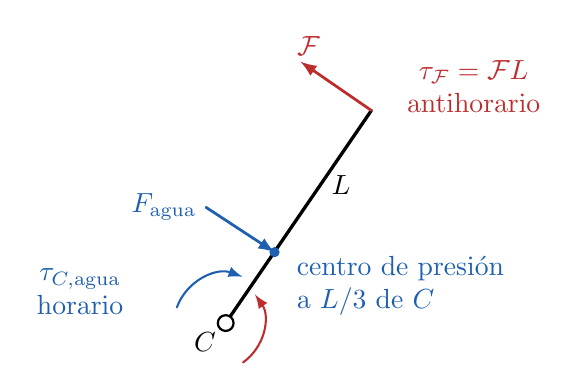
\begin{tikzpicture}[x=1cm,y=1cm,line cap=round,line join=round]
        \coordinate (C) at (3.40,0.55);
        \coordinate (S) at (5.25,3.25);
        \coordinate (CP) at (4.02,1.45);

        % Compuerta y articulación
        \draw[line width=1.2pt] (C) -- (S);
        \fill[white] (C) circle (0.10);
        \draw[line width=0.8pt] (C) circle (0.10);
        \node[below left] at (C) {$C$};
        \node[right] at (4.62,2.30) {$L$};

        % Fuerza externa en el extremo superior
        \draw[forcered,-latex,line width=1.0pt] (S) -- (4.35,3.87);
        \node[forcered,above] at (4.45,3.82) {$\mathcal{F}$};
        \node[forcered,align=center] at (6.55,3.55)
            {$\tau_{\mathcal F}=\mathcal{F}L$\\antihorario};

        % Resultante hidrostática y centro de presión
        \fill[hydroblue] (CP) circle (0.065);
        \draw[hydroblue,-latex,line width=1.0pt] (3.15,2.02) -- (CP);
        \node[hydroblue,left] at (3.15,2.02) {$F_{\mathrm{agua}}$};
        \node[hydroblue,right,align=left] at (4.18,1.02)
            {centro de presión\\a $L/3$ de $C$};
        \node[hydroblue,align=center] at (1.55,0.95)
            {$\tau_{C,\mathrm{agua}}$\\horario};

        % Sentidos de giro alrededor de C
        \draw[hydroblue,-latex,line width=0.75pt]
            (2.78,0.75) arc[start angle=160,end angle=70,radius=0.65];
        \draw[forcered,-latex,line width=0.75pt]
            (3.62,0.05) arc[start angle=-55,end angle=35,radius=0.62];

    \end{tikzpicture}
    \caption{Diagrama de torques de la compuerta respecto a la articulación $C$.}
\end{figure}
